\section{Floating environments in \LaTeX}
	Certain document elements, such as large tables and graphic diagrams, cannot be broken across pages. If placed directly in the text stream, they could leave awkward blank gaps at the bottom of pages.
	
	To resolve this, \LaTeX\ places them inside floating containers or \emph{floats}, allowing the compiler to move them to optimal page positions without breaking text flow. In other words, \LaTeX\ allows them to ``float'' across the document to optimum positions.
	
	There are two floating environments which are commonly used in \LaTeX:
	\begin{enumerate}
		\item The \lstinline|table| floating environment which is used to construct tables within the document.
		\item The \lstinline|figure| floating environment which is used to incorporate figures within the document.
	\end{enumerate}
	
	\paragraph{Position specifiers:} To guide \LaTeX\ as to the order of preference where we want the float to be laid out in the document, we can use any or a combination of the following optional placement parameters:
	\begin{itemize}
		\item \verb|h| for \emph{here} which tries to place it approximately at the location in the source code.
		\item \verb|t| for \emph{top} which tries to place it at the top of a page.
		\item \verb|b| for \emph{bottom} which tries to place it at the bottom of a page.
		\item \verb|p| for \emph{page} which tries to place it on a dedicated float-only page.
		\item \verb|!| for \emph{override} which tries to relaxe internal \LaTeX\ placement restrictions for float count and area.
	\end{itemize}
	For instance, when we combine the placement specifiers as \verb|htbp|, \LaTeX\ first tries to place the float at the location in the \emph{source code} (because of the \verb|h|). If that is not possible, then it tries to place the float at the \emph{top} of the current or next page (because of the \verb|t|). Again, if that is not possible, it tries to place the float at the \emph{bottom} of the current or next page (because of the \verb|b|). Finally, if all of the above fail, then it places the float on a \emph{page dedicated to floats} only (because of the \verb|p|), in the order in which they appear in the document.
	
	\paragraph{Captions, labels and referencing:} Given below are the macros which are available for including captions for the float, adding labels and referencing them elsewhere.
	\begin{itemize}
		\item \lstinline|\caption{text}| generates a numbered caption for the table or figure.
		\item \lstinline|\label{key}| assigns a symbolic key value to the element so that it can be referenced elsewhere. The \lstinline|\label| macro must always be placed below the \lstinline|\caption| macro.
		\item \lstinline|\ref{key}| and \lstinline|\pageref{key}| retrieve the float number and the page number where it currently appears in the document.
	\end{itemize}
	
	\subsection{Typesetting tables}
		\LaTeX\ allows us to typeset tables using the \lstinline|tabular| environment which is wrapped within a \lstinline|table| floating environment.
		
		The general syntax for using the \lstinline|tabular| environment is structured as follows:
\begin{lstlisting}
\begin{table}
	\caption{table caption}
	\label{key}
	\begin{tabular}[position]{column specifiers}
		{cell 11} & {cell 12} & {...} & {cell 1n} \\
		{cell 21} & {cell 22} & {...} & {cell 2n} \\
		{...} & {...} & {...} & {...} \\
		{cell m1} & {cell m2} & {...} & {cell mn} \\
	\end{tabular}
\end{table}
\end{lstlisting}
		
		\subsubsection{Column specifiers}
			This is a mandatory sequence of formatting characters defining the number, alignment and border layout of columns.
			\begin{itemize}
				\item \verb|l| for \emph{left}-aligned column.
				\item \verb|c| for \emph{centre}-aligned column.
				\item \verb|r| for \emph{right}-aligned column.
				\item | to insert a vertical gridline between adjacent columns.
				\item \verb|p{width}| for a fixed-width \emph{paragraph} column that automatically wraps multi-line text.
			\end{itemize}
		
		\subsubsection{Table body}
			The body of the table, which contains the rows and columns, has a syntax which requires the following elements:
			\begin{itemize}
				\item The column separator (\&) separates individual cells within a row.
				\item The row terminator (\verb|\\|) marks the end of a row. An optional length argument (e.g. \lstinline|\\[5pt]|) can be added to insert extra vertical space after a row.
				\item The full horizontal gridline (\lstinline|\hline|) draws a horizontal rule across the full width of the table.
				\item The partial horizontal gridline (\lstinline|\cline{i-j}|) draws a horizontal rule from column \verb|i| to column \verb|j| of the table.
			\end{itemize}
		
		\subsubsection{Vertical position}
			This is an optional argument which controls how the entire table aligns vertically relative to the baseline of the surrounding narrative text.
			\begin{itemize}
				\item \verb|c|, which is the default value, aligns the vertical \emph{centre} of the table with the text baseline.
				\item \verb|t| aligns the baseline of the \emph{top} row with the surrounding text baseline.
				\item \verb|b| aligns the baseline of the \emph{bottom} row with the surrounding text baseline.
			\end{itemize}
			
		For instance, the following code typesets a table:
\begin{lstlisting}
\begin{table}[h]
	\caption{Table of voltage and current observations}
	\label{tab:ohms-law}
	\begin{tabular}[t]{|c|c|c|c|}
		\hline
		\textbf{S. No.} & \textbf{Voltage (V)} & \textbf{Current (mA)} & \textbf{Resistance ($\Omega$)} \\ \hline
		{1} & {0.5} & {3.5} & {142} \\ \hline
		{2} & {1.0} & {6.7} & {149} \\ \hline
		{3} & {1.5} & {9.9} & {151} \\ \hline
		{4} & {2.0} & {13.1} & {153} \\ \hline
		{5} & {2.5} & {17.2} & {145} \\ \hline
	\end{tabular}
\end{table}
\end{lstlisting}
		which yields the following output:
		\begin{table}[h]
			\centering
			\caption{Table of voltage and current observations}
			\label{tab:ohms-law}
			\begin{tabular}[t]{|c|c|c|c|}
				\hline
				\textbf{S. No.} & \textbf{Voltage (V)} & \textbf{Current (mA)} & \textbf{Resistance ($\Omega$)} \\ \hline
				{1} & {0.5} & {3.5} & {142} \\ \hline
				{2} & {1.0} & {6.7} & {149} \\ \hline
				{3} & {1.5} & {9.9} & {151} \\ \hline
				{4} & {2.0} & {13.1} & {153} \\ \hline
				{5} & {2.5} & {17.2} & {145} \\ \hline
			\end{tabular}
		\end{table}
	
	\newpage
	\subsection{Formatting figures}
		To incorporate external vector graphics (e.g. PDF, EPS) or raster images (e.g. PNG, JPG), we can use the \lstinline|\includegraphics| macro which is provided by the \lstinline|graphicx| package.
		
		To use the \lstinline|graphicx| package, we include the following line in the preamble:
\begin{lstlisting}
\usepackage{graphicx}
\end{lstlisting}
		
		The general syntax for using the \lstinline|\includegraphics| macro is structured as follows:
\begin{lstlisting}
\begin{figure}
	\centering
	\includegraphics[key=value-list]{filename}
	\caption{table caption}
	\label{key}
\end{figure}
\end{lstlisting}
		
		The various arguments used are as follows:
		\begin{itemize}
			\item The mandatory argument \lstinline|filename| contains the relative or absolute path of the graphic file. The file extension (e.g. \verb|.png|, \verb|.jpg|, \verb|.pdf|, \verb|.eps|) can be omitted, as \LaTeX\ automatically searches for supported formats.
			\item The optional arguments \lstinline|key=value-list| is a comma-separated list of properties to resize, scale, rotate or trim the graphic. Some of the commonly used parameters are
			\begin{itemize}
				\item \lstinline|width| which resizes the image to a specific width (e.g. \lstinline|width=4.5cm| or \lstinline|width=0.8\textwidth|).
				\item \lstinline|height| which resizes the image to a specific height (e.g. \lstinline|height=3.6in| or \lstinline|width=0.5\textheight|).
				\item \lstinline|keepaspectratio| which prevents image distortion when both \lstinline|width| and \lstinline|height| are specified simultaneously.
				\item \lstinline|scale| which scales both width and height proportionally by a factor (e.g. \lstinline|scale=0.6| scales the image to 60\% of its size).
				\item \lstinline|angle| which rotates the image counter-clockwise by a specified angle in degrees (e.g. \lstinline|angle=45|).
				\item \lstinline|trim| which crops margins off the image as \lstinline|trim=left bottom right top| (e.g. \lstinline|trim=1cm 2cm 1cm 2cm|).
			\end{itemize}
		\end{itemize}
		
		\newpage
		For instance, the following code incorporates a figure in the file named \verb|schrodingers-cat.png| which is contained in a folder titled \verb|figures| that lies in the same location as the \LaTeX\ source code:
\begin{lstlisting}
\begin{figure}[h!]
	\centering
	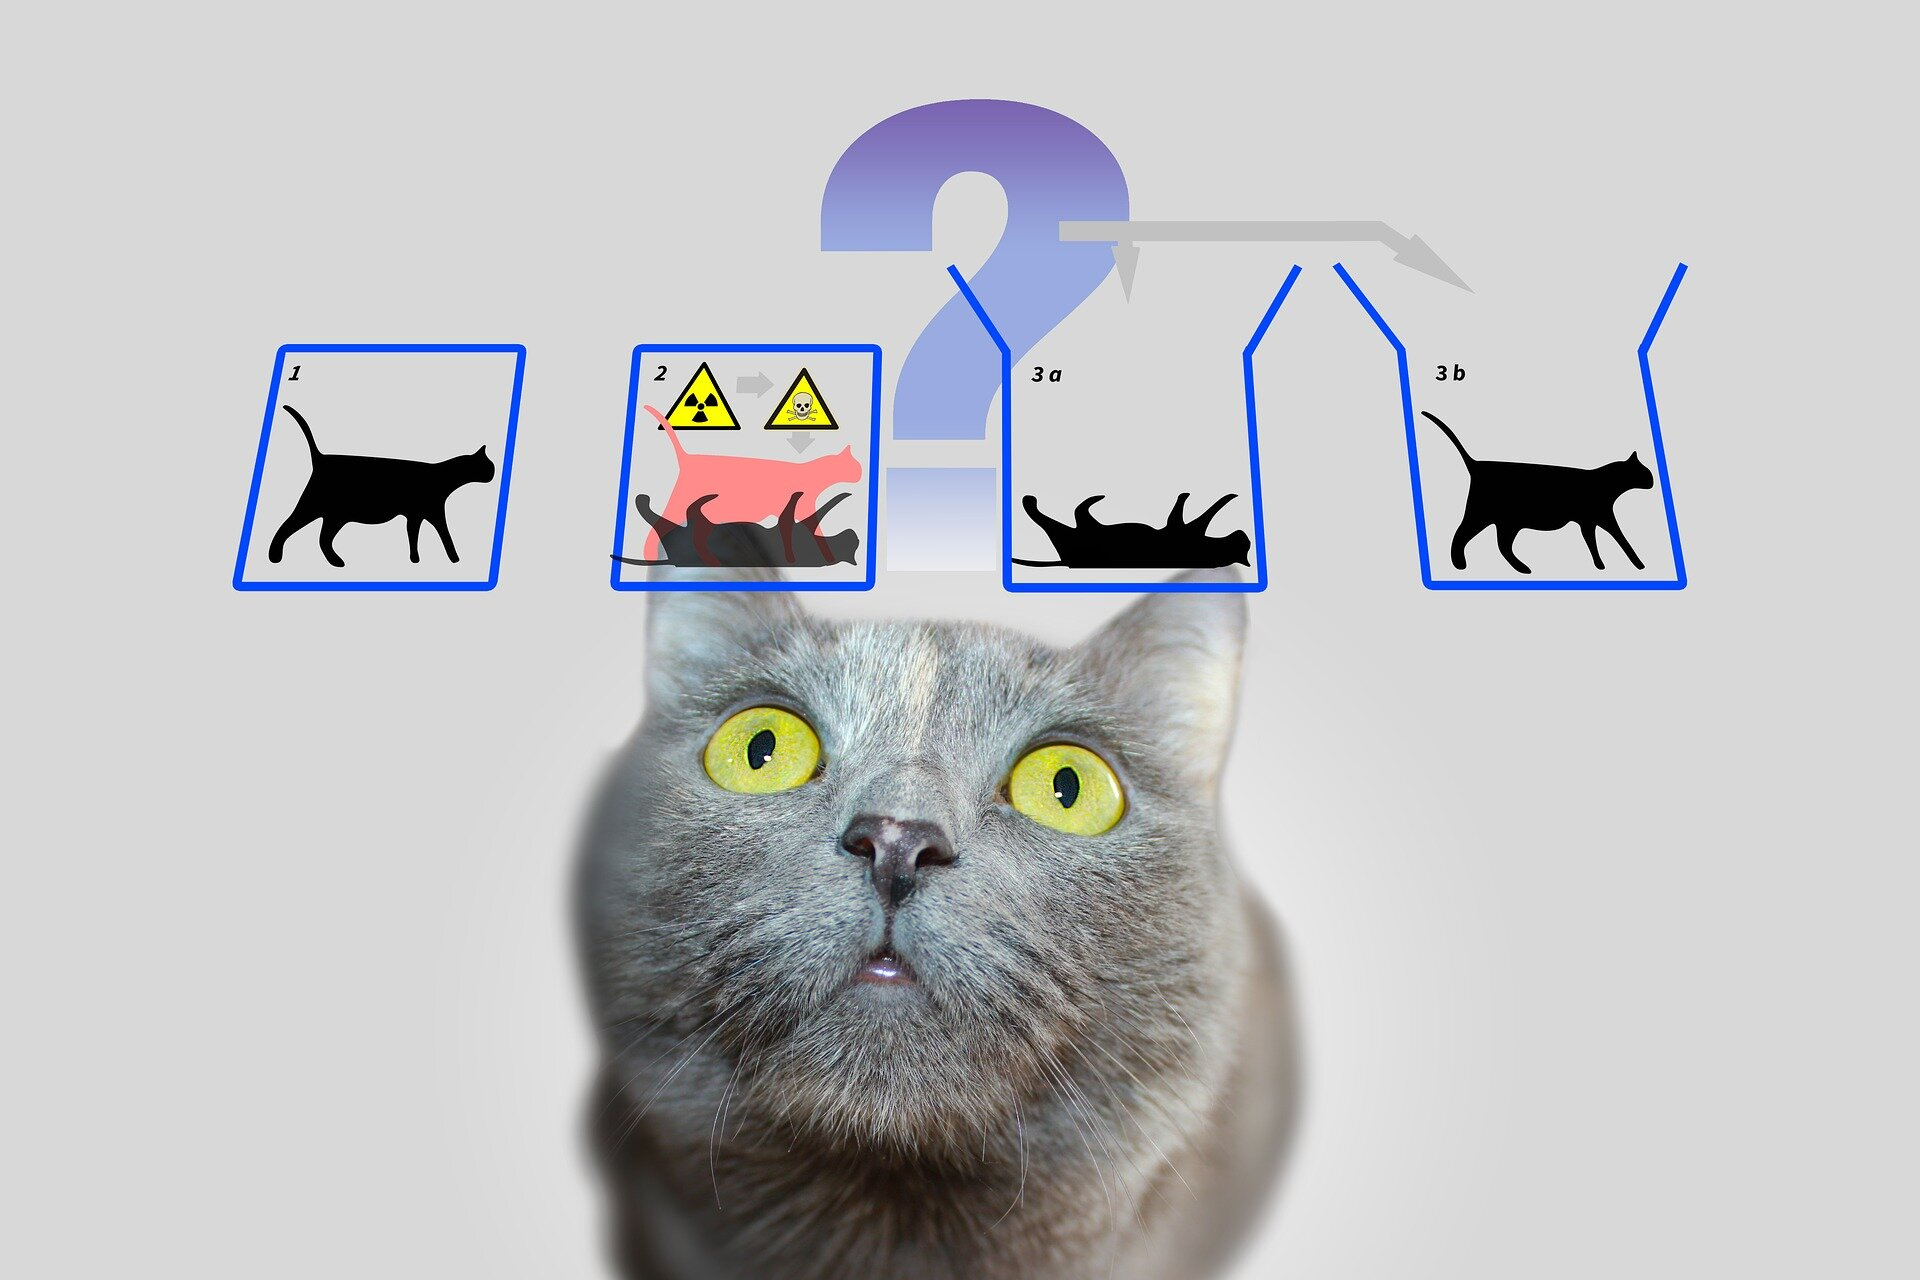
\includegraphics[width=0.4\textwidth, angle=30]{figures/schrodingers-cat}
	\caption{Schrodinger's cat}
	\label{fig:schrodinger-cat}
\end{figure}
\end{lstlisting}

		which yields the following output:
		
		\begin{figure}[h!]
			\centering
			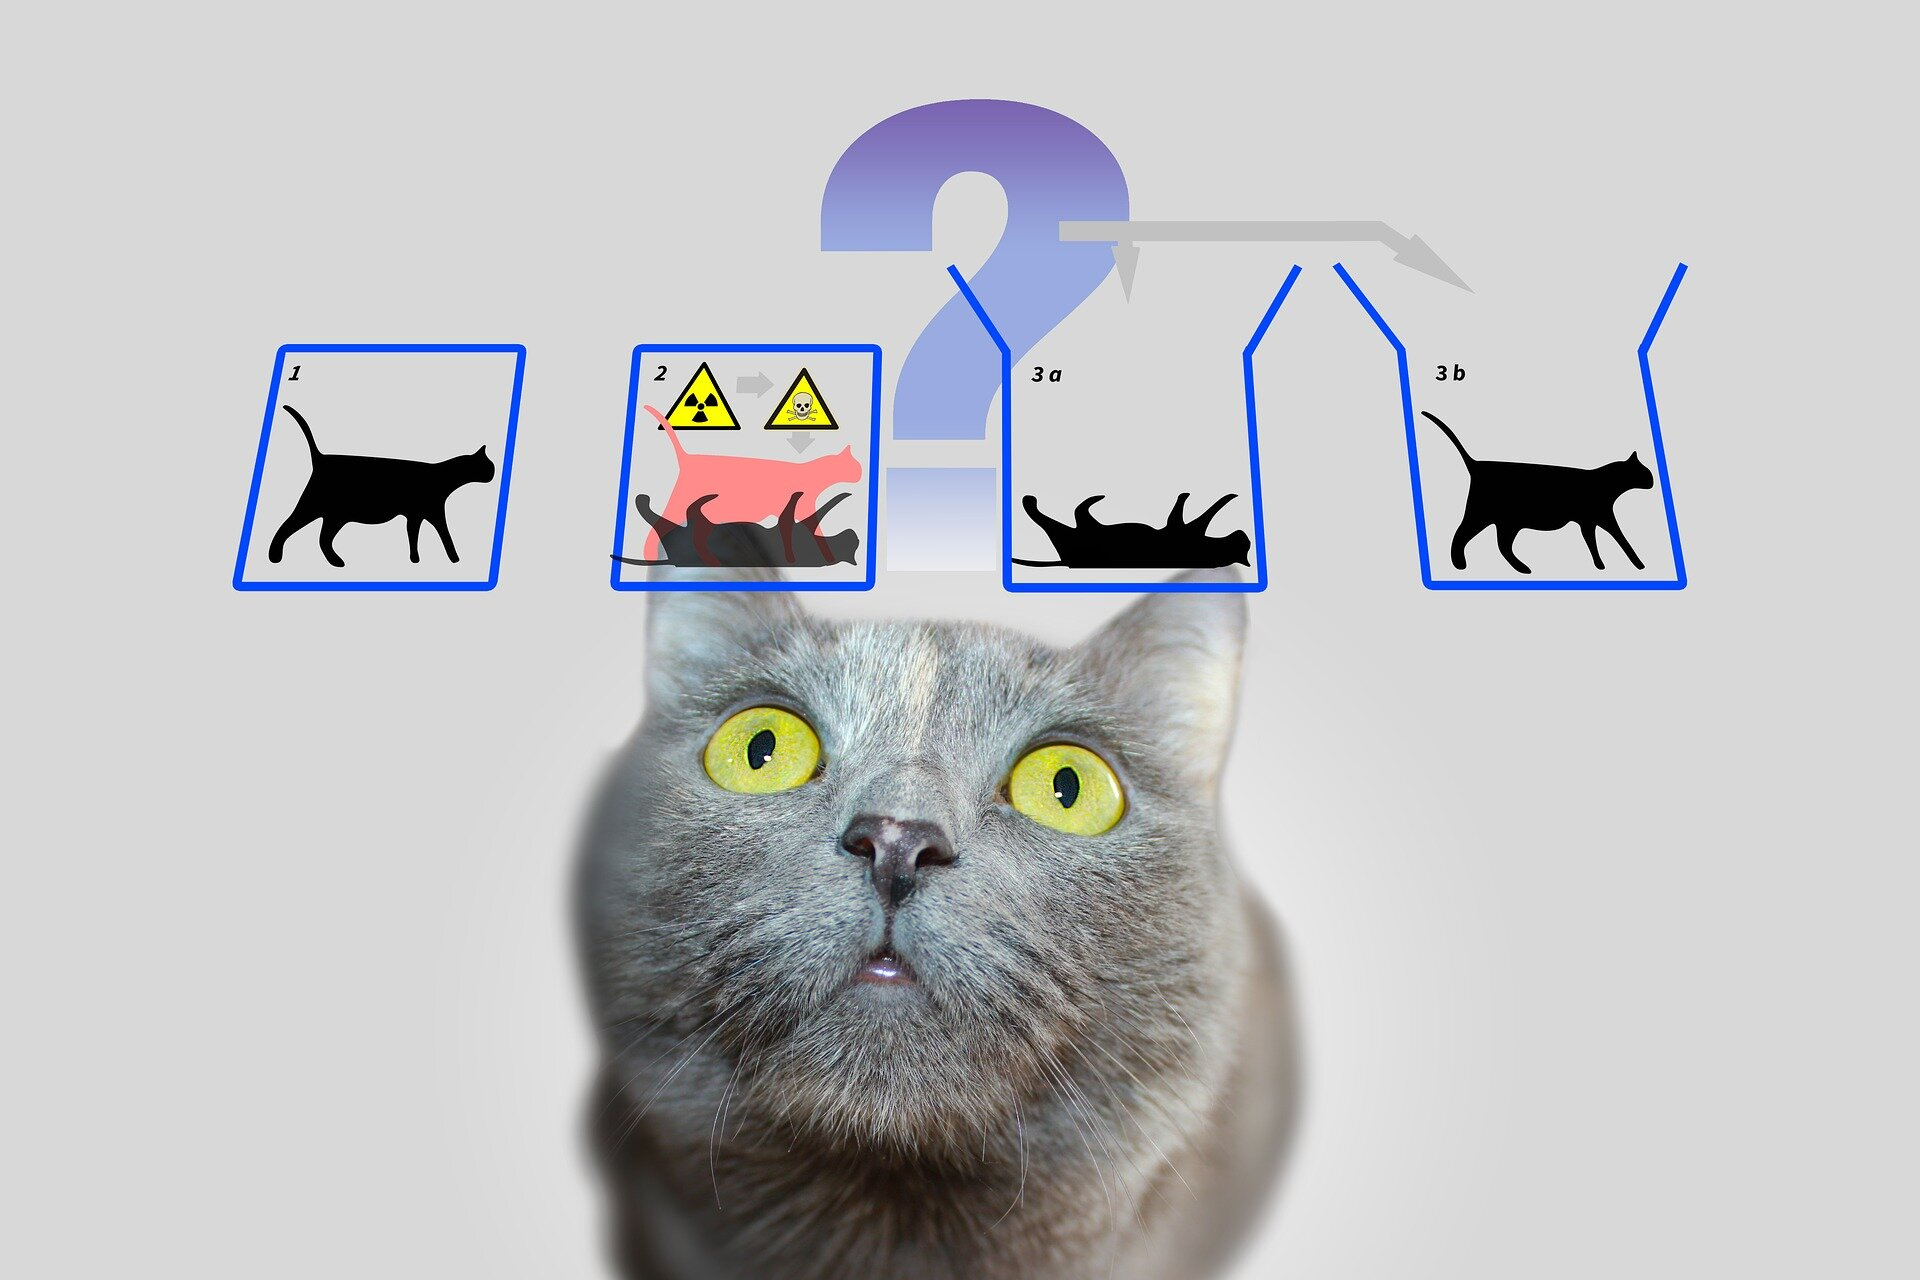
\includegraphics[width=0.4\textwidth, angle=30]{figures/schrodingers-cat}
			\caption{Schrodinger's cat}
			\label{fig:schrodinger-cat}
		\end{figure}